\documentclass[10pt]{article}

%% Various useful packages and commands from different sources

\usepackage[applemac]{inputenc}
\usepackage[english]{babel}
\usepackage[T1]{fontenc}
\usepackage{cite, url,color} % Citation numbers being automatically sorted and properly "compressed/ranged".
%\usepackage{pgfplots}
\usepackage{graphics,amsfonts}
\usepackage[pdftex]{graphicx}
\usepackage[cmex10]{amsmath}
\usepackage{bm}
% Also, note that the amsmath package sets \interdisplaylinepenalty to 10000
% thus preventing page breaks from occurring within multiline equations. Use:
 \interdisplaylinepenalty=2500
% after loading amsmath to restore such page breaks as IEEEtran.cls normally does.

% Compact lists
\usepackage{enumitem}
\usepackage{booktabs}
\usepackage{fancyvrb}

\usepackage{listings} % for Matlab code
\definecolor{commenti}{rgb}{0.13,0.55,0.13}
\definecolor{stringhe}{rgb}{0.63,0.125,0.94}
\lstloadlanguages{Matlab}
\lstset{% general command to set parameter(s)
framexleftmargin=0mm,
frame=single,
keywordstyle = \color{blue},% blue keywords
identifierstyle =, % nothing happens
commentstyle = \color{commenti}, % comments
stringstyle = \ttfamily \color{stringhe}, % typewriter type for strings
showstringspaces = false, % no special string spaces
emph = {for, if, then, else, end},
emphstyle = \color{blue},
firstnumber = 1,
numbers =right, %  show number_line
numberstyle = \tiny, % style of number_line
stepnumber = 5, % one number_line after stepnumber
numbersep = 5pt,
language = {Matlab},
extendedchars = true,
breaklines = true,
breakautoindent = true,
breakindent = 30pt,
basicstyle=\footnotesize\ttfamily
}

\usepackage{array}
% http://www.ctan.org/tex-archive/macros/latex/required/tools/
\usepackage{mdwmath}
\usepackage{mdwtab}
%mdwtab.sty	-- A complete ground-up rewrite of LaTeX's `tabular' and  `array' environments.  Has lots of advantages over
%		   the standard version, and over the version in `array.sty'.
% *** SUBFIGURE PACKAGES ***
\usepackage[tight,footnotesize]{subfigure}
\usepackage[top=2.2cm, bottom=2.2cm, right=1.7cm,left=1.7cm]{geometry}
\usepackage{indentfirst}


%\setlength\parindent{0pt}
\linespread{1}

\usepackage{mathtools}
\DeclarePairedDelimiter{\ceil}{\lceil}{\rceil}
\DeclarePairedDelimiter{\floor}{\lfloor}{\rfloor}
\DeclareMathOperator*{\argmax}{arg\,max}
\newcommand{\M} {\mathtt{M}}
\newcommand{\dB} {\mathrm{dB}}
\newcommand{\tr} {\mathrm{tr}}
\newcommand{\ofdM} {\mathcal{M}}
\newcommand{\DFTmat} {\mathbf{F}}
\newcommand{\lmod}[1] {_{\,\mathrm{mod}\,#1}}
\newcommand{\DFTreduced} {\mathbf{\tilde{F}}}



\graphicspath{ {figures/} }

% equations are numbered section by section
%\numberwithin{equation}{section}


\begin{document}
\title{Digital Transmission - Homework 4}
\author{Andrea Dittadi, Davide Magrin, Michele Polese}

\maketitle

%%%%%%%%%%%%%%%%%%%%%%%%%%%%%%%%%%%%%%%%%
%%%%%%%%%%%%%% PROBLEM 1 %%%%%%%%%%%%%%%%
%%%%%%%%%%%%%%%%%%%%%%%%%%%%%%%%%%%%%%%%%

\section*{Problem 1}

% Description of system setup

\begin{figure}
	\centering
	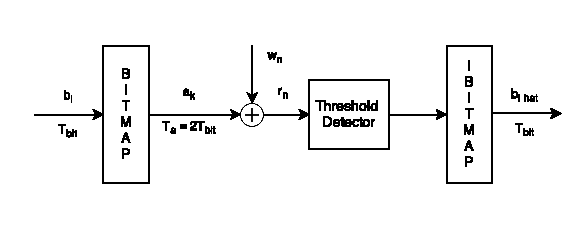
\includegraphics[width = 0.6\textwidth]{SC_uncoded}
	\caption{Block diagram for the simulation of a Single Carrier uncoded QPSK}
	\label{fig:problem1_scuncoded}
\end{figure}

\begin{figure}
	\centering
	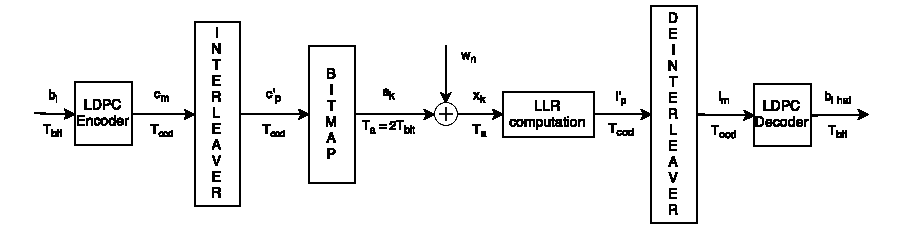
\includegraphics[width = \textwidth]{SC_coded}
	\caption{Block diagram for the simulation of a Single Carrier coded QPSK}
	\label{fig:problem1_sccoded}
\end{figure}

The uncoded Single Carrier QPSK configuration with ideal channel was implemented as described in Figure~\ref{fig:problem1_scuncoded}. First of all, a random data stream is created using the \texttt{randi} function. For the BER simulations, $L_{bits} = 2^{24}$ bits were used for every SNR. While this number of bits is unnecessarily large to estimate the Bit Error Rate for the lower SNRs, it was decided not to optimize it because the simulations were sufficiently fast. This is due to the lightweight operations the script has to perform: after the initial bitmapping of the bits to obtain the QPSK symbols, the channel only adds noise and there is no need to perform any convolution with an impulse response since the channel is ideal. Finally, the receiver only computes a thresholding and an inverse bit mapping. The results of the simulation can be seen in Figure~\ref{fig:problem1_pbit}, and coincide with those obtained in the previous homework. %TODO insert this reference to the old homework???

When using coding, the script has to perform more complex computations that are illustrated in Figure~\ref{fig:problem1_sccoded}. The random bit sequence needs to have a length compatible with both the encoder and the interleaver. In fact, the provided LDPC encoder requires information words to have length $L_{iw} = 32400$ bits, and encodes them into codewords of length $L_{cw} = 64800$ bits. This doesn't represent a limitation, as shorter information words may be padded to reach the desired length, encoded and de-padded at the receiver, once decoded. In order to simplify things, however, it was decided to only send information words that have length that is a multiple of the information word length required by the encoder. Additionally, the interleaver matrix was given dimensions of $30 \times 36$ in order to facilitate the process of interleaving the codeword bits. Since $30 \cdot 36 = 1080$ is a divisor of the length of the codewords, when codewords of length $L_{cw} = k \cdot 64800, k \in \mathbb{N^{+}}$ need to be interleaved, the interleaver uses a number of matrices equal to $\frac{L_{cw}}{30\cdot36} = 60 \cdot k$, thus ensuring that all matrices will be filled completely and that no additional padding is required. Using this setup, if the desired length is $L_d$, the nearest compatible length of the message to be sent can be computed using the expression $L_{msg} = \lceil \frac{L_{d}}{32400} \rceil \cdot 32400$. 
%% TODO give real number used 
Once the bits are generated, encoded and interleaved, they are translated into symbols with $\sigma_a^2 = 2$ using the QPSK bitmap and sent through the channel, that adds the noise $w_k \sim \mathcal{CN}(0, \sigma_w^2)$, given that the SNR of the channel is $\Gamma = \frac{\sigma_a^2}{\sigma_w^2}$. 

The receiver needs then the log-likelihood ratios in order to perform soft decoding. The received symbols are complex, but it is straightforward to extend the definition of LLR proposed in \cite{bc} for the case of binary real symbols in absence of ISI. In particular if the received symbol $x_k = a_k + w_k$ is real, with $a_k$ binary and the noise $w_k$ real Gaussian with variance $\sigma_I^2$, then the log-likelihood ratio LLR is defined in \cite{bc} as 
\begin{equation}
	\ell_k^{bin, real} = \frac{2 x_k}{\sigma_I^2}
\end{equation}
Let's now consider the QPSK case, which is the constellation used by tx-rc in this homework. Note that the bitmap maps the bits with even index ($2k$) to the real part of the $k$-th symbol, the bits with odd index ($2k + 1$) to its imaginary part. Let the received symbol be $x_k = a_k + w_k$, with $a_k = a_{k, I} + j a_{k, Q}$ a QPSK symbol and $w_k$ complex white noise with variance $\sigma_w^2$. Then let $x_{k,I}$ be the real part of $x_k$, i.e. $x_{k,I} = a_{k, I} + w_{k, I}$, with $w_{k,I}$ the noise per component with variance $\sigma_I = \sigma_w^2/2$, and $x_{k, Q}$ the imaginary part, i.e. once again $x_{k,Q} = a_{k, Q} + w_{k, Q}$ with $w_{k, Q}$ with variance $\sigma_I = \sigma_w^2/2$. 

At this point it is possible to define a log-likelihood ratio for the real part and the imaginary part of the symbol $x_k$, which are
\begin{equation}
	\ell'_p =
	\begin{dcases}
	\frac{2 x_{k,I}}{\sigma_I^2}, \quad p = 2k \\
	\frac{2 x_{k,Q}}{\sigma_I^2}, \quad p = 2k +1
	\end{dcases}
\end{equation}

%TODO: more about what the LLR is and on how it works? 

If the symbol period is $T_a$, the LLR vector will have bit period equal to $T_{cod} = \frac{T_a}{2}$, as one value of the LLR corresponds to one bit of the encoded message at the transmitter side. In order to get back to the actual correspondence with the original message $b_l$, it is necessary to deinterleave the LLR and to decode it. By feeding the LLR to the decoder, we are using it in its \emph{soft decoding} mode: the decoder will make use of the likelihood associated to the value of each bit, instead of the ``hard value'' of the bits, to perform the decoding. %TODO Necessary?
The output of the decoder, $\hat{b}_l$, is the final decision on the received symbols. This is the vector that is compared to $b_l$ in order to compute the probability of bit error. The results can once again be seen in Figure~\ref{fig:problem1_pbit}. 

% BER plot for coded vs uncoded QPSK
\begin{figure}
	\centering
	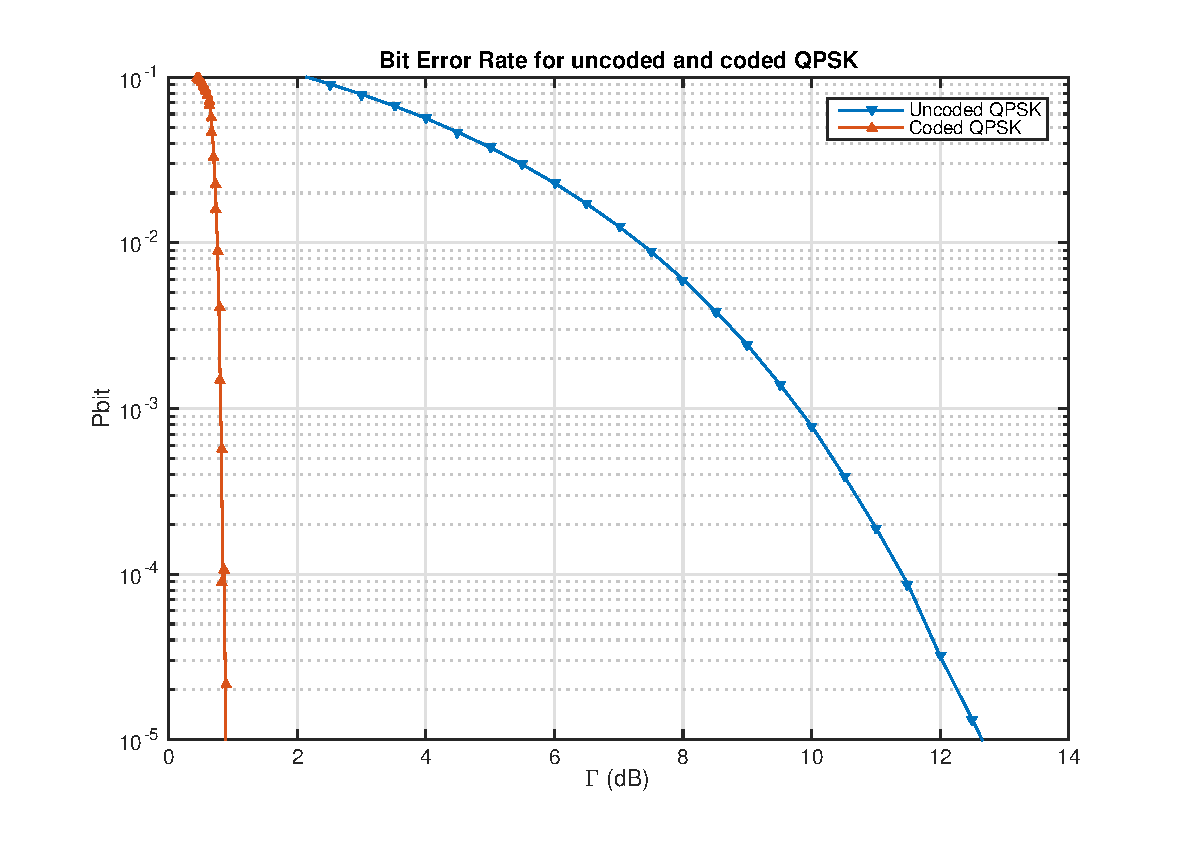
\includegraphics[width = 0.6\textwidth]{problem1}
	\caption{BER simulation results for coded vs. uncoded QPSK}
	\label{fig:problem1_pbit}
\end{figure}



%%%%%%%%%%%%%%%%%%%%%%%%%%%%%%%%%%%%%%%%%
%%%%%%%%%%%%%% PROBLEM 2 %%%%%%%%%%%%%%%%
%%%%%%%%%%%%%%%%%%%%%%%%%%%%%%%%%%%%%%%%%

\section*{Problem 2}
The setup used for the simulations with the DFE only varies when considering the coded and uncoded setting: using the actual or estimated impulse response only reflects changes on the DFE setting (i.e., the impulse response and the noise variance). 

The simulations that do not use channel coding follow the block scheme in %Figure~\ref

The timing phase $t_0 = 5$ was determined as the index of the first non-zero sample of the channel impulse response ${h_i}$.

% Required stuff:
% Setting of the DFE (as of the previous homework)
% In the HW text it is said that this should be re-designed for every SNR, specify this is what we do (the values of sigma_w are needed by the DFE and vary for each of the SNRs)
% Write values of t0, M1, M2 and D used. Say that these will be used for every SNR
% Write expressions of LLRs for the known channel, specifying that the noise that is being taken into account is the actual channel noise. There also is no ISI noise as it is assumed to have been cancelled by the DFE, specify this!
% Write expression of LLRs for the estimated channel. Specify that we use the estimated channel noise, as it is the only thing the receiver actually knows. 



\begin{figure}
	\centering
	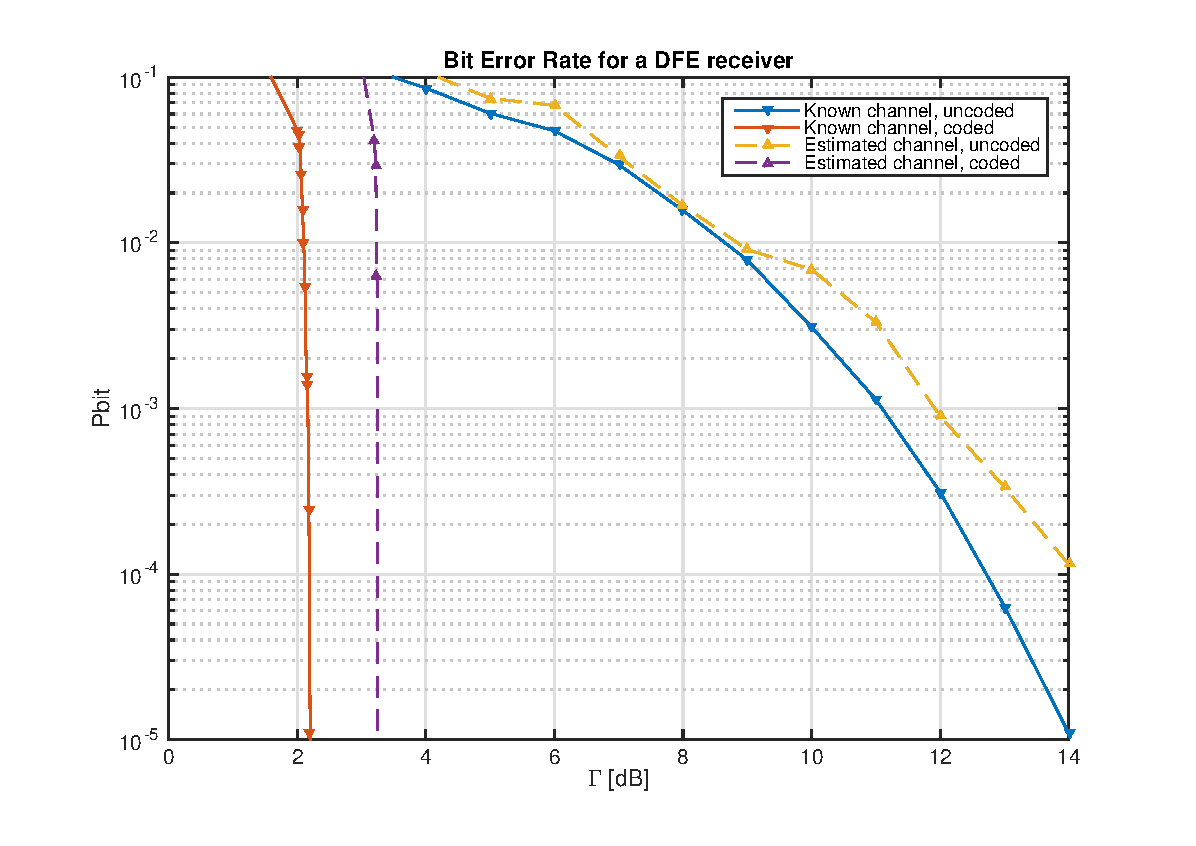
\includegraphics[width = 0.6\textwidth]{problem2}
	\caption{BER simulation for a DFE receiver using the estimated and actual channel ir, with or without coding}
	\label{fig:problem2_pbit}
\end{figure}

%%%%%%%%%%%%%%%%%%%%%%%%%%%%%%%%%%%%%%%%%
%%%%%%%%%%%%%% PROBLEM 3 %%%%%%%%%%%%%%%%
%%%%%%%%%%%%%%%%%%%%%%%%%%%%%%%%%%%%%%%%%
\section*{Problem 3}

\begin{figure}
	\centering
	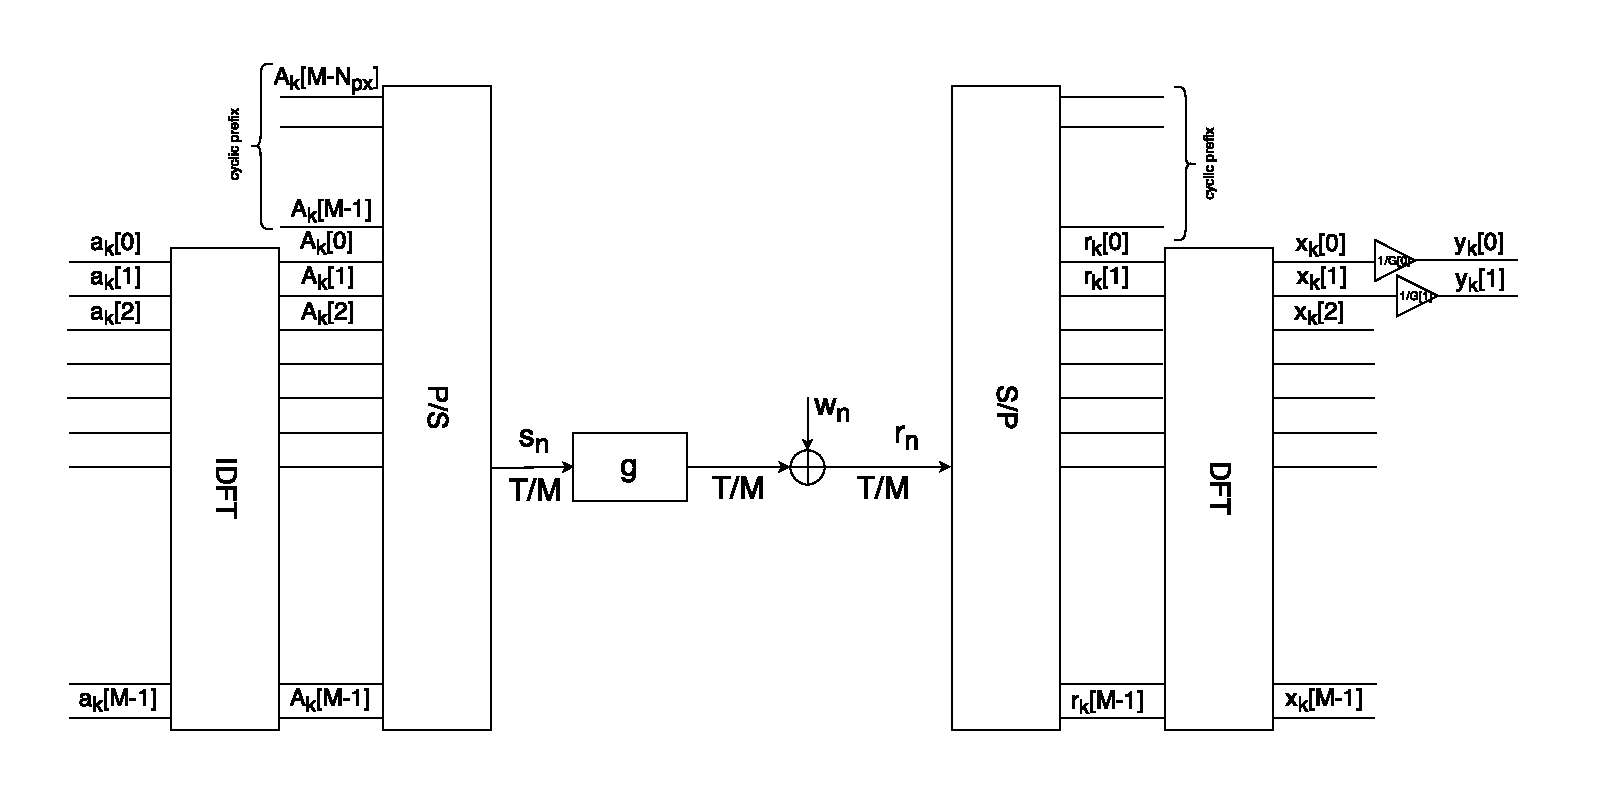
\includegraphics[width = 0.8\textwidth]{OFDM}
	\caption{OFDM system structure}
	\label{fig:OFDM}
\end{figure}

\subsection*{Transmitter structure}
Figure~\ref{fig:OFDM} shows the structure of an OFDM transmitter-receiver and a model for the channel. The symbols denoted by $a_k$ could represent either coded or uncoded bits, as in previous problems. The block index is called $k$. The symbols are taken in chunks of $\ofdM = 512$ in order to compose the vector $a_k[i], i \in [0, \ofdM - 1]$. The IDFT is then computed to get $A_k[i], i\in [0, \ofdM-1]$. At this point a cyclic prefix (whose role will be explained after having introduced the receiver) is inserted, i.e. for each block the last $N_{px} = 7$ symbols are repeated at the beginning of the vector $A_k$. Finally, the symbols $A_k[i]$ are serialized and sent through the channel as part of the signal $s_n$.

% Consideration on SNR
As usual the SNR is defined as $\Gamma = \frac{\sigma_s^2 E_h}{\sigma_w^2}$, however in an OFDM system the meaning of $\sigma_s^2$ changes. As mentioned, the transmitter performs an IDFT, which is
\begin{equation}
	A_k[\ell] = \frac{1}{\ofdM} \sum_{i = 0}^{\ofdM - 1} W_{\ofdM}^{-i\ell} a_k[i], \quad \ell = 0, 1, \dots, \ofdM-1,
\end{equation}
therefore we have 
% see formula 9.35, 9.38, 9.39
\begin{equation}
	\sigma_s^2 = \dfrac{\sigma_a^2}{\ofdM}.
\end{equation}
To compute the power of the noise introduced by the channel we must then consider the SNR as
\begin{equation}
	\Gamma = \dfrac{\sigma_a^2 E_h}{\ofdM \sigma_w^2},
	\label{eq:snrOFDM}
\end{equation}
which yields
\begin{equation}
	\sigma_w^2 = \dfrac{\sigma_a^2 E_h}{\ofdM \Gamma}.
\end{equation}

\subsection*{Receiver structure}
The structure of the receiver of OFDM is illustrated in Fig.~\ref{fig:OFDM}. The timing phase is $t_0 = 5 T$, and corresponds to the beginning of reception of the cyclic prefix by the receiver. For each block of $\ofdM + N_{px}$ symbols, the first $N_{px}$ are discarded, and the DFT is then computed only on the $\ofdM$ samples that do not belong to the cyclic prefix of that block. Let the vector of received symbols in block $k$ (before the DFT is performed) be $\mathbf{r}_k$, and let $\mathbf{g}_{c,\ofdM}$ be the channel impulse response, of length $N \le N_{px} + 1$, padded with zeros in order to have a vector of length $\ofdM$. Then it is possible to define the circulant matrix of the IDFT of the transmitted symbols $a_k[i], i = 0, \dots, \ofdM$ as
\begin{equation}
	\boldsymbol{\Xi} = 
	\begin{bmatrix}
		A_k[0] & A_k[\ofdM - 1] & \dots & A_k[1] \\
		A_k[1] & A_k[0] & \dots & A_k[2] \\
		\vdots & \vdots & \ddots & \vdots \\
		A_k[\ofdM - 1] & A_k[\ofdM - 2] & \dots & A_k[0] \\
	\end{bmatrix}
\end{equation}
and express $\mathbf{r}_k$ as
\begin{equation}
	\mathbf{r}_k = \boldsymbol{\Xi} \mathbf{g}_{c,\ofdM} + \mathbf{w}_k
\end{equation}
with $\mathbf{w}_k$ a vector of AWGN samples. %TODO variance? has this w been defined before?
The receiver then performs the DFT using an $\ofdM \times \ofdM$ DFT matrix $\DFTmat$, and since $\boldsymbol{\Xi}$ is a circulant matrix, the result can be written as
\begin{equation}
	 \mathbf{x}_k = \DFTmat \mathbf{r}_k = \DFTmat \boldsymbol{\Xi} \DFTmat^{-1} \DFTmat \mathbf{g}_{c,\ofdM} + \DFTmat \mathbf{w}_k = \mathrm{diag}\{\mathbf{a}_k\} \mathbf{G}_c + \mathbf{W}_k.
\end{equation}
The vector $\mathbf{W}_k$ is a still composed of independent Gaussian random variables, each with variance $\sigma_W^2 = \ofdM \sigma_w^2$. 

This procedure removes the effects of ICI and ISI introduced by the non-ideal channel, and it is followed by a scaling of the received symbols on each channel in order to get the same constellation of the transmitter. More specifically, for each subchannel $i$ we have
\begin{equation}
	y_k[i] = \frac{x_k[i]}{G_c[i]} = a_k[i] + \frac{W_k[i]}{G_c[i]}
	\label{eq:yofdm}
\end{equation}
Finally the receiver performs a decision. If the transmitted bits are uncoded, it uses a threshold detector on each subchannel and an inverse bitmap. Note that the performances of an uncoded OFDM system are negatively affected by the presence of subchannels with a small frequency response coefficient $G_c[i]$. In fact, in those subchannels the received symbols are below noise level, and the noisy term in $y_k[i]$ is amplified by a factor $(G_c[i])^{-1}$.

Instead, if coding is used, the data that would be lost because of the attenuation of its subchannel can be recovered. In particular, given the observed symbol $y_k[i]$ defined in~\eqref{eq:yofdm}, let the variance per component of the noise affecting $y_k[i]$ be
\begin{equation}
	\sigma_I^2 = \frac{\sigma_W^2}{2 |G_c[i]|^2} = \frac{\ofdM \sigma_w^2}{2 |G_c[i]|^2}.
\end{equation}
Then the log-likelihood ratios (LLR) of each subchannel for the pair of bits that are mapped in each symbol are defined as
\begin{equation}
\ell'_p[i] =
	\begin{dcases}
	\frac{2\Re(y_k[i])}{\sigma_I^2} = 2\Re(y_k[i]) \frac{|G_c[i]|^2 }{0.5 \ofdM \sigma_w^2}, \quad p = 2k \\
	\frac{2\Im(y_k[i])}{\sigma_I^2} = 2\Im(y_k[i]) \frac{|G_c[i]|^2 }{0.5 \ofdM \sigma_w^2}, \quad p = 2k+1 \\
	\end{dcases}
\end{equation}
%% TODO check indices

\subsection*{Channel estimation for OFDM}
In order to perform the operations described in the previous section, the receiver has to know the frequency response of the channel and the noise power of each subchannel. In this homework the simulation of the BER has been carried out both with an \textit{a priori} perfectly known channel and with an estimated channel. 

%TODO give reasons behind this kind of spacing
The estimation of the channel has to be performed with $L_{ts} = 32$ pilot symbols, using one single block, for instance $k=0$. In \eqref{eq:snrOFDM} the power of the transmitted symbols is usually $\sigma_a^2 = 2$, but the pilot symbols have power $\sigma_{ts}^2 = 4$ as required. The pilot symbols $a_{ts}[i]$ are transmitted on the $L_{ts}$ subchannels with indices
\begin{equation}
	i \in \mathcal{T}_{ind} = \{q \frac{\ofdM}{L_{ts}}, \, q = 0,\ldots,L_{ts}-1 \}  = \{ 0, 16, 32, \dots, 496 \},
\end{equation}
i.e. with a spacing of $\ofdM/L_{ts}$ subchannels between each other. The other $\ofdM - L_{ts}$ symbols can be data or anything else, since they are not used for the estimation. At the receiver, after the DFT, each of the $L_{ts}$ symbols $x_0[i], i \in \mathcal{T}_{ind}$ is divided by the corresponding pilot symbol $a_{ts}[i]$ in order to get $\tilde{G}[i]$. Formally, the estimated frequency response of the $i$-th subchannel is
\begin{equation}
	\tilde{G}[i] = \dfrac{x_0[i]}{a_{ts}[i]} = \dfrac{a_{ts}[i] G_c[i] + W_0[i]}{a_{ts}[i]} = G_c[i] + \dfrac{W_0[i]}{a_{ts}[i]}, \qquad i \in \mathcal{T}_{ind}.
\end{equation}

Our estimation method exploits the fact that the channel impulse response can have at most $N_{px} + 1 = 8$ taps, so the uncorrelated samples of the frequency response $G_c[i]$ are at most 8. In the presence of noise, however, the estimated frequency response has more than 8 degrees of liberty, and we will try to determine a better estimate (more robust to noise), by using all 32 symbols, equally spaces as described above.

Let $\DFTmat$ be a $\ofdM \times \ofdM$ DFT matrix as before, and let $\DFTmat'$ be the result of keeping only the first $N_{px}+1$ columns of $\DFTmat$. Defining $\mathbf{G}_c = [ G_c[i] ]_{i = 0,\ldots,\ofdM-1}$ as the DFT of the channel impulse response, then
\begin{equation}
	\mathbf{G}_c = \DFTmat \cdot \mathbf{g}_{c,\ofdM} = \DFTmat' \cdot \mathbf{g}_c.
\end{equation}
By choosing the 32 subchannels with pilot symbols (i.e. for $ i \in \mathcal{T}_{ind}$) we define a matrix $\DFTreduced$ of size $L_{ts} \times N_{px} + 1$ as the result of selecting the rows $ i\in \mathcal{T}_{ind} $ of matrix $\DFTmat'$.. Let 
\begin{equation}
\mathbf{\tilde{W}} = \left[ \dfrac{W_0[i]}{a_{ts}[i]} \right] _{i\ \in \mathcal{T}_{ind}}
\end{equation}
be the vector of noise samples corresponding to the considered subchannels (i.e. the ones we are using to transmit the pilot symbols). Then it is possible to write $\mathbf{\tilde{G}}_c$ as
\begin{equation}
	\mathbf{\tilde{G}}_c = \DFTreduced \cdot \mathbf{g}_{c} + \mathbf{\tilde{W}}.
	\label{eq:OFDMfreqresp}
\end{equation}

Given an observation $\boldsymbol{\Omega}$ of the vector $\tilde{\mathbf{G}}_c = [ \tilde{G}[i] ]_{i\in \mathcal{T}_{ind}}$ the vector $\mathbf{g}_{c}$ can be finally computed by applying the LS method, which is formulated as
\begin{equation}
	\mathbf{\hat{g}}_c = \arg\min_{\mathbf{g}_c} ||\DFTreduced \cdot \mathbf{g}_{c} - \boldsymbol{\Omega}||^2.
\end{equation}
In matrix form, the solution is given by the following equations:
\begin{align}
	\boldsymbol{\Phi} &= \DFTreduced^H \DFTreduced \\
	\boldsymbol{\theta} &= \DFTreduced^H \boldsymbol{\Omega} \\ 
	\hat{\mathbf{g}}_{c} &= \boldsymbol{\Phi}^{-1} \boldsymbol{\theta}.
\end{align}
Finally, let $\hat{\mathbf{g}}_{c, \ofdM}$ be $\hat{\mathbf{g}}_{c}$ with a zero padding in order to make it $\ofdM$ samples long, as defined before. In order to estimate the frequency response at each subchannel, the DFT is applied on $\hat{\mathbf{g}}_{c, \ofdM}$, to obtain $\mathbf{\hat{G}}_c = \mathcal{F}[\mathbf{\hat{g}}_{c, \ofdM}]$. 

In conclusion, the noise power is estimated as 
\begin{equation}
	\hat{\sigma}_w^2 = \frac{1}{L_{ts}} \sum_{i \in \mathcal{T}_{ind}} |a_{ts}[i]\hat{G}_c[i] - x_0[i]|^2
\end{equation}
provided that $a_{ts}[i]\hat{G}_c[i] - x_0[i]$ has zero mean.


\subsection*{Alternative method dunno}

In absence of noise, \eqref{eq:OFDMfreqresp} can easily be inverted to obtain the exact value of $\mathbf{g}_c$. In fact, that equation represents a system of 32 equations in 8 unknowns, which is an overdetermined system with a unique solution. In fact, we could in principle use any 8 subchannels to get an estimated frequency response -- we tried different scenarios and the resulting estimate is as good as we want, provided a high enough SNR. The presence of noise affects the variances of the estimator: more precisely, the variance of the estimate $\hat{G}_c[i]$, that only depends on the noise, gets very high for subchannel indices $i$ that are far from the nearest element of the set $\mathcal{T}_{ind}$. For this reason, the solution of equally spaced subchannels for the estimation is the most robust to noise.

As already mentioned, the frequency response we are estimating has only 8 degrees of liberty, therefore in principle we could use for instance 8 equally spaced subchannels to get a good result. Moreover, for the same reason, the 512 coefficients $G_c[i]$ are heavily correlated, therefore adjacent subchannels will have similar frequency response. The last observation suggests that a good solution for the estimation of the subchannel noise would be to transmit training symbols on adjacent subchannels, and measure the variance of the estimated frequency responses $\hat{G}_c[i]$, assuming in those subchannels $G_c[i]$ is approximately constant. Indeed, if the noise is powerful enough, the variability of the estimated $\hat{G}_c[i]$ is almost completely due to noise.

%TODO Spiegare bene come funziona, selezionando varianze e mediandole, poi scalamenti vari..

The main tradeoff of this method is the following. Using larger groups of subchannels we are increasing the accuracy of the variance estimation, but there are two downsides. Firstly, the variability of the frequency response starts playing a major role in the estimated variance, yielding a worse estimation of the noise variance that does not prevail anymore. Secondly, we are increasing the spacing between groups of subchannels, therefore the estimation of the frequency response itself gets worse. On the other hand, using small groups, the estimated variance would be mainly due to noise, and the frequeny response estimation would be more accurate, but we have too few samples in each group to compute the sample variance.

Using 8 groups of 4 subsequent subchannels, the implementation is easy, we get a good estimate of the frequency response, and the estimate of the noise power is strongly improved with respect to our original method, up until SNR = 18 dB approximately. These performance results are discussed below.

%TODO Discuss performances (comparison script)

\begin{thebibliography}{10}

\bibitem{bc}
Benvenuto, Cherubini, Algorithms for Communications Systems and their Applications, Wiley, 2004

\end{thebibliography}

\end{document}
